\chapter{Implementazione}\label{ch:implementazione}

\section{Tecnologie utilizzate}\label{sec:tecnologie-utilizzate}
Per la realizzazione del framework non sono state utilizzate librerie esterne se non ScalaTest e
Scalafmt~\cite{scalafmt} - opportunamente configurato - per la formattazione del codice.
Si segnala inoltre che, a causa dell'incompatibilità con Scala 3, è stata utilizzata la libreria JaCoCo~\cite{jacoco}
invece di Scoverage.
Infine, non avendo individuato alcuna alternativa, non è stato possibile utilizzare Scalafix.

\section{Suddivisione del lavoro}\label{sec:suddivisione-del-lavoro}
In questa sezione viene illustrata la suddivisione del lavoro e le parti di progetto realizzate da ciascun membro del
gruppo.

\subsection{Cavalieri}\label{subsec:giacomo-cavalieri}
Il mio compito principale è stato quello di realizzare i \texttt{ComponentTag}, \texttt{CListTag},
e il \texttt{ComponentsContainer} descritto precedentemente alla Sezione~\ref{sec:container-di-componenti}.
Inoltre ho collaborato con i miei colleghi alla realizzazione delle \texttt{CList}.

\subsubsection{CList}
Nelle prime fasi di sviluppo ho cercato di risolvere il problema del garantire la type-safety dei sistemi.
Mi sono inizialmente documentato su possibili meccanismi forniti dal linguaggio individuando nell'utilizzo delle
tuple una possibile soluzione.
Infatti, in Scala 3 le tuple possono fungere da meccanismo per ottenere liste eterogenee di elementi
preservando informazioni sul loro tipo~\cite{tuples}.
Tuttavia, questo ha comportato alcuni problemi come l'impossibilità di garantire a tempo di compilazione che le tuple
fossero composte di soli elementi sottotipi di \texttt{Component}
(\textit{i.e.} data la tupla $(T_1,\dots,T_n)$ garantire che $T_i <: \text{Component } \forall i=1,\dots,n$).
Per questo, prendendo ispirazione dall'approccio utilizzato nella libreria Shapeless~\cite{shapeless},
ho individuato una possibile soluzione nell'adozione delle \texttt{CList}, realizzate in seguito
da Farabegoli con il mio aiuto.

\subsubsection{ComponentTag}
Il framework realizzato utilizza in maniera pervasiva informazioni sui tipi dei componenti, necessarie
per la loro memorizzazione e manipolazione.
Per questo è stato realizzato il \texttt{ComponentTag}, ovvero un oggetto che mantiene informazioni riguardo
al tipo a tempo di compilazione di un componente;
in questo modo è stato possibile raggruppare componenti con lo stesso tipo inferito all'interno del
\texttt{ComponentsContainer}.

Un altro aspetto fondamentale tenuto in considerazione è stato quello di garantire una certa semplicità di
utilizzo della libreria.
Infatti, sarebbe stato poco pratico per un utente dover specificare manualmente i \texttt{ComponentTag}
come argomenti dei metodi che ne necessitano la conoscenza.
Per ovviare a tale problema si sono sfruttati alcuni meccanismi avanzati offerti da Scala 3:
in particolare l'uso di \textit{macro}, \textit{inlining} e i nuovi \textit{impliciti}.

Tramite un semplice import (\texttt{import dev.atedeg.ecscala.given}) l'utente non deve preoccuparsi
della presenza dei \texttt{ComponentTag} che saranno generati automaticamente dal compilatore tramite
un'apposita macro riportata nel Listato~\ref{lst:component-tag}.

\lstinputlisting[label={lst:component-tag}, caption=Macro per la generazione di un \texttt{ComponentTag}.]
{code/component-tag.sc}

\subsubsection{CListTag}
In maniera analoga a quanto discusso per i \texttt{ComponentTag}, è stato definito un tag generato dal
compilatore tramite macro per le \texttt{CList}.
Infatti, è risultato fondamentale sfruttare la metaprogrammazione per effettuare controlli aggiuntivi
a livello di compilazione sulla correttezza delle \texttt{CList}.
Per esempio, non dev'essere possibile specificare una lista di
componenti con tipi ripetuti nella definizione di un sistema;
ciò non avrebbe senso dato che un'entità può avere al più un componente per tipo e si vuole impedire tale situazione
al momento della compilazione.

L'implementazione di tali controlli è riportata al Listato~\ref{lst:clist-tag}.
\lstinputlisting[label={lst:clist-tag}, caption=Macro e controlli per la generazione di un \texttt{CListTag}.]
{code/clist-tag.sc}

\subsubsection{Deletable CLists}\label{subsubsec:deletable}
Un sistema definito per alcuni tipi di componenti $T_{C1},\dots,T_{Cn}$ deve ritornare nel proprio metodo
\texttt{update} una \texttt{CList} di componenti dello stesso tipo che verranno usati per aggiornare lo stato
delle entità su cui il sistema può essere applicato.
Durante il processo di sviluppo è sorta la necessità di poter indicare la rimozione di un particolare componente
dall'entità: per esempio, il sistema di un videogioco che opera su entità dotate del componente \texttt{LifePoints}
potrebbe voler rimuovere tale componente una volta che questo scende a 0.

Utilizzare dei valori opzionali per indicare la rimozione o meno di un componente
(\eg \texttt{Some(???)~\&:~None~\&:~CNil}) avrebbe comportato una
riscrittura delle \texttt{CList} in modo tale da poter accettare valori opzionali.

Una soluzione, a mio avviso più elegante, ha sfruttato due nuovi meccanismi introdotti in Scala 3:
i \textit{match types}~\cite{match-types} e gli \textit{union types}~\cite{union-types}.
Come mostrato nel Listato~\ref{lst:deletable} una versione ``deletable'' di una \texttt{CList}
\texttt{T1~\&:~...~\&:~TN~\&:~CNil} non è altro
che la lista stessa dove ogni elemento \texttt{Ti} viene sostituito da uno union type \texttt{(Ti | Deleted)}.
Dato che un tipo \texttt{T} è sottotipo di \texttt{T | Other} una \texttt{CList} sarà sottotipo della sua
equivalente versione \texttt{Deletable}.

Così facendo l'utente può continuare a specificare una lista di componenti come valore di ritorno del metodo
\texttt{update} dei sistemi;
una sostanziale differenza sta nel fatto che, al posto di un qualunque componente, potrà specificare
il componente speciale \texttt{Deleted} ad indicare che il componente in tale posizione è
stato cancellato (\eg \texttt{C1~\&:~Deleted~\&:~CNil} indica che il secondo componente deve essere eliminato
durante l'aggiornamento di stato dell'entità).

\lstinputlisting[label={lst:deletable}, caption=Implementazione del tipo \texttt{Deletable[L~<:~CList]}]
{./code/deletable.scala}

\subsection{Di Domenico}\label{subsec:nicolò-di-domenico}

Il mio ruolo nel progetto è stato principalmente quello d'implementare le \texttt{View} e i \texttt{System}, nonché
applicare ove necessario eventuali ottimizzazioni per rispettare il requisito non funzionale~\ref{itm:nf1}.

\subsubsection{View}

Essendo le \texttt{View} ed \texttt{ExcludingView} progettate come indicato in Figura~\ref{fig:view}, si è rivelato
utile costruire un iteratore astratto che permettesse di fattorizzare tutto il codice comune.
In particolare si noti come la \texttt{ExcludingView} itera su un sottoinsieme delle entità ritornate dalla stessa
\texttt{View}, che invece non esprime vincoli di esclusione di componenti.
Per questo motivo è stato creato il \texttt{BaseViewIterator}, che si occupa di recuperare dal
\texttt{ComponentsContainer} tutte le mappe che associano ciascuna entità all'istanza (se presente) del componente di
ciascun tipo.
Infine, partendo da tali mappe, si occupa di testare l'appartenenza alla view di ciascuna entità e, in caso affermativo,
estrarne tutti i componenti richiesti.

Una semplice ottimizzazione utilizzata per rendere più veloce l'iterazione di una \texttt{View} consiste
nell'individuare la mappa di componenti con meno elementi;
una volta trovata, si iterano tutte le entità contenute al suo interno e per ognuna si controlla che sia presente in
tutte le altre mappe.
In caso affermativo, si procede all'estrazione di tutti i suoi componenti richiesti.

\begin{figure}
    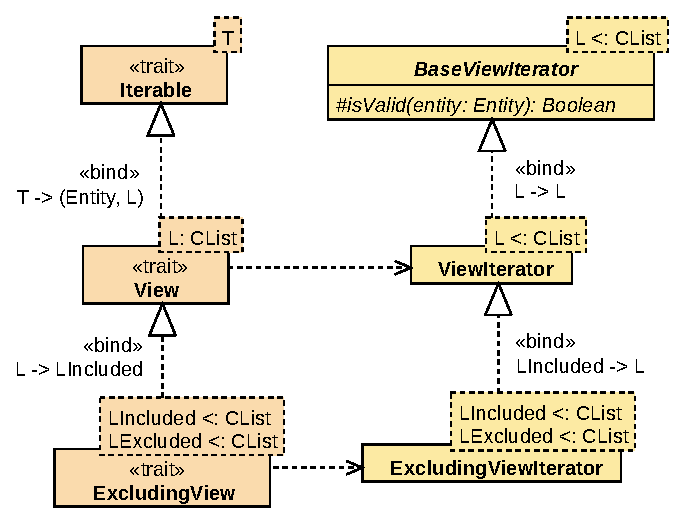
\includegraphics{./img/View}
    \caption{Design di dettaglio di \texttt{View} ed \texttt{ExcludingView}}
    \label{fig:view}
\end{figure}

\subsubsection{System}

Un \texttt{System} è un blocco di codice che può essere aggiunto al \texttt{World} e viene chiamato a ogni aggiornamento
di stato della simulazione.
Ogni \texttt{System} ha due metodi:
\begin{itemize}
    \item \texttt{shouldRun}: metodo booleano che indica se il \texttt{System} dev'essere eseguito
    \item \texttt{update}: metodo che contiene il codice arbitrario da eseguire
\end{itemize}

Su di esso sono stati costruiti \texttt{IteratingSystem} ed \texttt{ExcludingSystem}, due wrapper type-safe
rispettivamente per \texttt{View} ed \texttt{ExcludingView}.
Questi due sistemi definiscono i seguenti metodi:
\begin{itemize}
    \item \texttt{shouldRun}: metodo booleano che indica se l'\texttt{IteratingSystem} dev'essere eseguito
    \item \texttt{before}: metodo eseguito prima di iterare su tutte le entità con i componenti richiesti
    \item \texttt{update}: metodo eseguito per ciascuna entità contenente le operazioni da effettuare sui suoi
    componenti richiesti
    \item \texttt{after}: metodo eseguito dopo aver iterato su tutte le entità con i componenti richiesti
\end{itemize}

Il metodo \texttt{update} deve ritornare una \texttt{CList} dei nuovi componenti;
grazie all'utilizzo delle \texttt{CList} (descritte in dettaglio nella sottosezione~\ref{sec:lista-di-componenti})
verrà verificato a tempo di compilazione che i nuovi componenti abbiano lo stesso tipo di quelli su cui opera il
sistema.
Per permettere la cancellazione di alcuni dei componenti, è stato implementato un match type chiamato
\texttt{Deletable[L~<:~CList]} descritto nella Sottosezione~\ref{subsubsec:deletable}.

L'\texttt{ExcludingSystem} è completamente analogo all'\texttt{IteratingSystem}, in quanto cambia solo la \texttt{View}
usata per ottenere le entità sulle quali iterare.

\subsection{Farabegoli}\label{subsec:farabegoli}
Il contributo apportato al progetto ha toccato buona parte del core del framework, nonché lo sviluppo dei benchmark.
Mi sono infine occupato della gestione del repository, della CI, dei rilasci del framework e della qualità del codice.

\subsubsection{CList}
La parte che mi ha conivolto in prima persona è stata la realizzazione delle \texttt{CList}.
Le \texttt{CList} rappresentano una parte fondamentale del framework realizzato, quindi è stato importante realizzare
diversi test per cercare d'individuare possibili errori.
Un esempio significativo riguarda i test effettuati sulla corretta destrutturazione di una \texttt{CList}: in questo
ambito si è rilevato un bug nella suite ScalaTest;
per una trattazione dettagliata del problema si veda la Sezione~\ref{sec:problemi-riscontrati}.

\subsubsection{World ed Entity}
Una delle parti che ho seguito nelle prime fasi di sviluppo è stata l'implementazione del \texttt{World} e delle
\texttt{Entity}.
In particolare mi sono occupato di definire l'interfaccia di entrambe le classi e di fornire una prima implementazione
di base.
Ho quindi implementato il codice necessario affinché ogni entità avesse un identificativo univoco all'interno del mondo.
Infine, mi sono occupato dello sviluppo dei test per la verifica delle classi oggetto d'implementazione.

\subsubsection{View}
Ho definito e implementato parzialmente la classe \texttt{View}: in particolare, ne ho realizzato l'interfaccia e
fornito una prima implementazione.
Sempre seguendo un approccio test-driven, ho realizzato anche i test necessari alla verifica del corretto funzionamento
delle classi sopra descritte.
Nell'ambito dello sviluppo delle view, Cavalieri e Di Domenico hanno sviluppato una macro per costruire la
view in modo che operi sui componenti effettivi passati nel generico;
in questa fase ho contribuito fornendo consigli e suggerimenti per una migliore implementazione del codice.

\subsubsection{Benchmarks}
Il requisito non funzionale~\ref{itm:nf1} fornisce una linea di base delle prestazioni che il framework deve rispettare;
a tal proposito ho definito una serie di benchmark per misurare le prestazioni di \texttt{View}, \texttt{System} e
dell'aggiornamento del \texttt{World}.
Mediante questi benchmark è stato possibile validare il requisito non funzionale sulla base di dati oggettivi.
Per una descrizione più approfondita dei benchmark si faccia riferimento alla Sezione~\ref{sec:benchmark}.

\subsection{Vitali}\label{subsec:linda-vitali}
All'interno del team, oltre a quello di sviluppatrice, ho svolto anche il ruolo di \textit{Product Owner}.
Dunque, mi sono occupata di supervisionare l'organizzazione del processo di sviluppo e di redigere
\textit{Product Backlog} e \textit{Sprint Backlog} al termine dei meeting, riportando quanto accordato insieme agli
altri membri.
Per quanto riguarda la parte di sviluppo del codice, mi sono occupata di una prima implementazione della classe
\texttt{Component}, del \texttt{ComponentsContainer} in collaborazione con Cavalieri e dell'\texttt{ECScalaDSL}.

\subsubsection{Component}\label{subsubsec:component-desc}
\texttt{Component} è il trait che un utilizzatore del framework deve estendere per implementare le caratteristiche delle
proprie \texttt{Entity}.
Contiene il riferimento alla \texttt{Entity} a cui è stato aggiunto e un
\textit{extension method}~\cite{extensionmethods} per permettere la conversione in \texttt{CList}.

\subsubsection{ComponentsContainer}\label{subsubsec:components-container}
Il \texttt{ComponentsContainer} descritto nella Sezione~\ref{sec:container-di-componenti} fornisce metodi per:
\begin{itemize}
    \item Aggiungere \texttt{Component} a una \texttt{Entity}
    \item Rimuovere \texttt{Component} da una \texttt{Entity}
    \item Rimuovere \texttt{Entity}
    \item Ottenere tutte le \texttt{Entity} e i rispettivi \texttt{Component}
\end{itemize}
Sebbene inizialmente fosse stata utilizzata una \texttt{HashMap} come struttura dati, in seguito si è optato per una
\texttt{AnyRefMap}, la quale, come descritto nella documentazione ufficiale~\cite{anyRefMap},
è ``\textit{notevolmente più veloce di una HashMap}''.
Infatti, come si può osservare in Tabella~\ref{tab:componentscontainer-benchmark}, ha contribuito nel rispettare il
requisito non funzionale~\ref{itm:nf1}.

\subsubsection{ECScalaDSL}\label{subsubsec:dsl-impl}
La realizzazione del DSL si è basata sulla necessità di rendere l'utilizzo del framework il più intuitivo possibile,
permettendo d'implementare le funzionalità di base del framework in un linguaggio che appaia simile alla lingua
inglese, come mostrato nel Listato~\ref{lst:dsl-withComp} e nel Listato~\ref{lst:dsl-view}.
Per farlo, ci si è ispirati al DSL \texttt{Matchers}~\cite{matchers} di ScalaTest.

Per utilizzare la sintassi specifica e le parole chiave del DSL, l'utente deve estendere il trait \texttt{ECScalaDSL},
abilitare le conversioni implicite (tramite \texttt{import scala.language.implicitConversions}) e importare i given del
framework\\(con \texttt{import dev.atedeg.ecscala.given}).

\lstinputlisting[
    label={lst:dsl-withComp},
    caption=Esempio scritto con \texttt{ECScalaDSL} di creazione di un \texttt{World} che contiene una \texttt{Entity}
    con i rispettivi \texttt{Component}.
]{code/dsl-withComp.scala}

\lstinputlisting[
    label={lst:dsl-view}, caption=Esempio scritto con \texttt{ECScalaDSL} di come ottenere una \texttt{View} dal
    \texttt{World} con uno specifico \texttt{Component} escludendone un altro.
]{code/dsl-view.scala}

Le funzionalità del DSL sono state implementate facendo largo uso dei metodi come operatori infissi in modo tale
da rendere il codice simile a una frase.
Inoltre, sono stati utilizzati i seguenti meccanismi di Scala 3:
\begin{itemize}
    \item \textbf{Extension methods:} utilizzato per abilitare sulla classe \texttt{Entity} i metodi
    \texttt{withComponents} e sulla classe \texttt{World} i metodi \texttt{hasAn} e \texttt{hasA}.
    Inoltre, è stato applicato il pattern \textit{Pimp My Library} per il metodo \texttt{withComponent} di
    \texttt{Entity} e per abilitare metodi di aggiunta e rimozione con operatori a entrambe le classi sopracitate
    \item \textbf{Context functions~\cite{contextfunctions}:} la funzionalità si è rivelata particolarmente utile per il
    metodo \texttt{hasA}, usato per aggiungere un \texttt{System} al \texttt{World}.
    Come si può notare nel Listato~\ref{lst:dsl-ctxf}, il metodo prende in ingresso una \textit{context function} che va
    da \texttt{World} a \texttt{Unit}.
    Il questo modo il \texttt{World} viene passato implicitamente alla funzione che lo utilizza permettendo l'aggiunta
    del \texttt{System}
    \item \textbf{Conversioni implicite:} sono state implementate due conversioni implicite\\
    \texttt{componentToClist[C~<:~Component:~ComponentTag]:\\Conversion[C,~C~\&:~CNil]}
    e \texttt{Conversion[Entity,~Seq[Entity]]} per evitare overloading di metodi
\end{itemize}

\lstinputlisting[
    label={lst:dsl-ctxf},
    caption=Esempio di utilizzo di una context function nel metodo \texttt{hasA}.
]{code/dsl-ctxf.scala}

Si è utilizzata una \textit{Type Class} \texttt{From} per realizzare la parte di sintassi che permette di effettuare
arbitrarie operazioni su \texttt{World} e \texttt{Entity} con il metodo \texttt{from} (parola chiave del DSL).
Come si può vedere nel diagramma in Figura~\ref{fig:from} è possibile specificare il tipo al quale si applica il metodo
\texttt{from} e il suo tipo di ritorno.
In questo modo, si può implementare la classe specifica per abilitare la sintassi necessaria di caso in caso.

\begin{figure}[H]
    \centering
    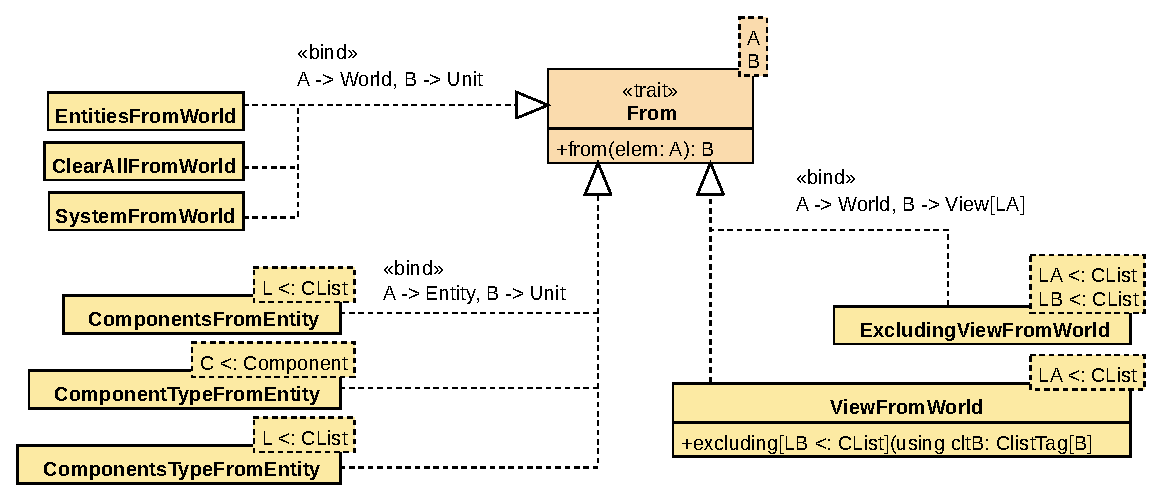
\includegraphics[width=\textwidth]{./img/From}
    \caption{Diagramma delle classi che mostra l'implementazione della type class \texttt{From}.}
    \label{fig:from}
\end{figure}

\section{Benchmark}\label{sec:benchmark}
Il requisito non funzionale~\ref{itm:nf1} richiede che il framework soddisfi un certo livello di prestazioni;
per questo motivo è stato necessario quantificare oggettivamente quali fossero le effettive prestazioni raggiunte.
I benchmark sono uno strumento piuttosto efficace per valutare i tempi di esecuzione (e non solo), fornendo
una stima delle prestazioni in gioco.

Con il termine benchmark si intende un insieme di test specifici per misurare le prestazioni di un software o computer.
Al termine dell'esecuzione del benchmark si ottiene un indice indicativo delle prestazioni che il sistema in oggetto ha
raggiunto.
I benchmark possono essere raggruppati in due categorie:
\begin{itemize}
    \item Sintetici (o microbenckmark): vanno a misurare le prestazioni di alcune parti specifiche di un sistema
    \item Applicativi: misurano le prestazioni complessive di un sistema, ad esempio di un'applicazione
\end{itemize}

Scrivere benchmark che misurano correttamente le prestazioni di solo una piccola parte di software è difficile: ci sono
diverse ottimizzazioni che la JVM e l'hardware sottostante sono in grado di fare quando il benchmark
esegue solo il componente~\cite{jmh:details}, ma tali ottimizzazioni non possono essere effettuate quando il componente
è eseguito come parte dell'intera applicazione, producendo dati falsati.
Implementazioni errate di benchmark possono far credere che le prestazioni dei componenti siano migliori di quanto non
siano in realtà.

È quindi necessario ricorrere a un framework di benchmarking apposito per ottenere misurazioni affidabili.
Si è scelto di utilizzare Jmh~\cite{jmh} per implementare i microbenchmark necessari alla verifica del
requisito non funzionale~\ref{itm:nf1}.

Il framework consente di definire in modo piuttosto semplice ma altamente configurabile i benchmark, come mostrato nel
Listato~\ref{lst:lstinputlisting4}.

\lstinputlisting[label={lst:lstinputlisting4}, caption=Codice per eseguire il setup di un benchmark.]
{code/benchmark.scala}

Alcuni parametri rilevanti nella configurazione dei benchmark sono:
\begin{itemize}
    \item \texttt{@Warmup}: si specifica quante iterazioni devono essere eseguite ``a vuoto'' prima di effettuare i
    test effettivi;
    questa procedura risulta necessaria dal momento che, quando si esegue per la prima volta un programma sulla JVM, la
    cache risulta vuota e quindi il caricamento iniziale delle classi è più lento.
    Eseguendo più volte la stessa porzione di codice si ``stabilizza'' la cache, quindi gli accessi successivi saranno
    più veloci e uniformi.
    Inoltre, nelle JVM HotSpot, l'interprete tiene traccia del numero di volte che un metodo viene eseguito: se tale
    numero supera una certa soglia allora viene identificato come \textit{hot method} (metodo che tipicamente ha dei
    loop) e quindi è \textit{JIT compiled}~\cite{jmh:details}.
    Chiamate successive all'ottimizzazione risulteranno quindi più veloci ed efficienti.
    In questo modo si garantisce che le misurazioni successive alla fase di warm up abbiano valori simili senza essere
    influenzate da condizioni esterne.
    \item \texttt{@Measurement}: si specifica quante volte il benchmark debba essere ripetuto.
    Per ogni esecuzione viene annotato il tempo impiegato e al termine dell'esecuzione viene riportato il tempo medio
    che impiega il test.
\end{itemize}

\subsection{Risultati}\label{subsec:risultati}
In Tabella~\ref{tab:system-benchmark} sono riportati i risultati riguardanti i \textit{System}, in cui si può osservare
che con $10\;000$ entità un sistema impiega mediamente cinque millisecondi a effettuarne l'aggiornamento, quindi il
requisito~\ref{itm:nf1} è ampiamente rispettato.
In Tabella~\ref{tab:componentscontainer-benchmark} sono riportati invece i risultati riguardanti il
\texttt{ComponentsContainer}, sia nella sua versione mutabile che immutabile.

\begin{table}[htp]
    \centering
    \begin{tabular}{c c}
        \toprule
        Numero entità & Tempo (ms) \\ \midrule
        1024 & $0.502 \pm 0.007$ \\
        2048 & $1.013 \pm 0.018$ \\
        4096 & $2.258 \pm 0.054$ \\
        10'000 & $5.413 \pm 0.074$ \\
        \bottomrule
    \end{tabular}
    \caption{Risultati benchmark sui \System.}\label{tab:system-benchmark}
\end{table}

\begin{table}[htp]
    \centering
    \begin{tabular}{c c c c}
        \toprule
        Numero entità & Tempo (ms) (imm.) & Tempo (ms) (mut.) & Speedup \\ \midrule
        1024 & $0.771 \pm 0.003$ & $0.498 \pm 0.002$ & $1.548 \pm 0.012$ \\
        2048 & $1.603 \pm 0.007$ & $0.969 \pm 0.004$ & $1.654 \pm 0.014$ \\
        4096 & $3.341 \pm 0.015$ & $2.224 \pm 0.014$ & $1.502 \pm 0.016$ \\
        10'000 & $8.216 \pm 0.047$ & $5.416 \pm 0.034$ & $1.517 \pm 0.018$ \\
        \bottomrule
    \end{tabular}
    \caption{Risultati benchmark sul \texttt{ComponentsContainer}}\label{tab:componentscontainer-benchmark}
\end{table}

A fronte dei risultati ottenuti dai benchmark si può affermare che il framework fornisce buone prestazioni con un
discreto numero di entità.

\section{Problemi riscontrati}\label{sec:problemi-riscontrati}

\subsection{Scalatest}\label{subsec:scalatest}
Nella libreria ScalaTest è stato riscontrato un bug nella sintassi \texttt{shouldNot typeCheck}.
Tramite questa espressione, dovrebbe essere possibile verificare che una porzione di codice, specificata come stringa,
non compili a causa di un errore nel processo di type checking.
Questo controllo risulta utile nel verificare la corretta destrutturazione delle~\texttt{CList} tramite
pattern matching.
In particolare si è verificato, tramite il codice riportato nel Listato~\ref{lst:lstinputlisting22}, che la
destrutturazione di una \texttt{CList} di dimensione diversa da quanto atteso porti ad un errore di compilazione.
A tal proposito si è definito il test indicato nel Listato~\ref{lst:lstinputlisting22}:
\lstinputlisting[
    label={lst:lstinputlisting22},
    caption=Test per la verifica dell'unpacking delle \texttt{CList}.
]
{./code/scalatest-bug.scala}
La prima asserzione verifica che la destrutturazione fallisca se si specificano meno elementi di quanti siano
effettivamente presenti nella lista;
nella seconda si testa lo scenario opposto, ovvero che la destrutturazione fallisca se la lista contiene meno elementi
di quanti ne sono stati specificati nel pattern matching.
Sebbene in entrambi i casi ci si aspetta che le espressioni non compilino a causa di errori nella fase di
type checking, questo non accade e le espressioni vengono erroneamente valutate come valide.
Il bug è stato segnalato agli sviluppatori della libreria mediante una issue~\cite{scalatest-bug}.

\subsection{Cross-building per Scala.js}\label{subsec:cross-building-per-scala.js}
Sin dalle prime fasi di sviluppo si è abilitata la modalità di \textit{cross-building}~\cite{cross-building} affinché il
framework venisse compilato anche per Scala.js~\cite{scalajs}.
Questo ha generato una serie di falsi errori all'interno dell'IDE (IntelliJ).
Infatti se si eseguivano i comandi di Sbt per la compilazione del progetto, quest'ultimo non sollevava alcun errore.
A tal proposito è stata aperta una issue~\cite{intellij-issue} sul bug tracker di Jetbrains.
Per una maggiore agilità nella scrittura del codice si è quindi scelto di rimuovere la cross-building dal progetto.

\subsection{System Builder}\label{subsec:system-builder}
La funzione di \texttt{update} di un sistema specifica diversi parametri (il \texttt{World} in cui il sistema è
eseguito, la \texttt{View} contenente tutte le entità, i componenti dell'entità che sta venendo modificata, eccetera);
tuttavia, spesso l'implementazione del metodo \texttt{update} necessiterà di solo alcuni dei parametri elencati.
Per questo motivo, inizialmente si è cercato di realizzare un builder che permettesse di costruire dinamicamente la
firma della funzione richiesta per costruire il sistema, permettendo una sintassi simile a quella riportata al
Listato~\ref{lst:builder-syntax}.

\lstinputlisting[label={lst:builder-syntax}, caption=Sintassi del builder per la creazione di sistemi.]
{./code/builder-syntax.sc}

Questo ha portato a individuare un problema nel compilatore Dotty che ha impedito di portare a compimento un simile
builder.
Infatti, a causa del problema, sarebbe stato necessario indicare un'annotazione di tipo nei parametri della
funzione la cui firma è stata costruita dinamicamente (un esempio è riportato al Listato~\ref{lst:builder-syntax-bug});
questo avrebbe comportato la scrittura di codice particolarmente verboso in contrasto con l'intento originale che aveva
portato a ideare tale builder.

Il bug~\cite{dotty-bug} è stato segnalato nelle issue del repository GitHub del compilatore Dotty
ed è stato recentemente risolto.

\lstinputlisting[
    label={lst:builder-syntax-bug},
    caption={Sintassi effettiva del builder,
    si notino le annotazioni di tipo ridondanti ma necessarie per la compilazione del codice.}
]
{./code/builder-syntax-bug.sc}
